\section{scrum artifacts}

\subsection{product backlog}
\begin{itemize}
  \item the Product Backlog is a list of functional and nonfunctional requirements
  \item it will deliver the vision of maximizing the ROI (glossary)
  \item is prioritized so that the items most likely to generate value are top priority and is divided into proposed releases
  \item changes in the Product Backlog reflect changing business requirements and how quickly or slowly the Team can transform Product Backlog into functionality.
  \item it is never complete
  \item is merely an initial estimate of the requirements
  \item is dynamic, evolves as the product and the environment does
  \item provides the Product Owner with a powerful tool for directing the project, giving the highest priority to the requirements that are of highest value to the business
  \item one of the purposes of the plan is to convince someone to fund the project, it should provide sufficient details to satisfy a source of funding that the project has merit, that it will deliver certain things at certain times, that the benefits outweigh the costs and risks, and that the people who will staff the project are sufficiently compentent to execute the plan
\end{itemize}

\begin{figure}[H]
  \centering
  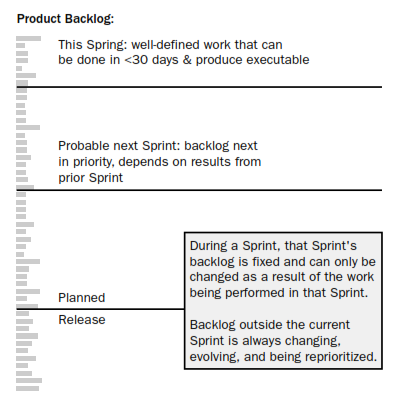
\includegraphics[width=0.6\textwidth]{./figures/product_backlog.PNG}
  \caption{product backlog}
  \label{fig:product_backlog}
\end{figure}\bigskip


\subsection{Sprint Backlog}
\begin{itemize}
  \item defines the work, or tasks, that a Team defines for turning the Product Backlog it selected for that Sprint into an increment of potentially shippable product functionality.
  \item Team compiles an initial list of these tasks in the second part of the Sprint planning meeting
  \item each takes should take roughly 4 to 16 hours to finish
  \item tasks taking longer than 4 to 16 hours are considered mere placeholders for tasks
  \item real-time picture of the work that the Team plans to accomplish
\end{itemize}


\subsection{Increment of Potentially Shippable Product Functionality}
\begin{itemize}
  \item Scrum requires Teams to build an increment of product functionality every Sprint
  \item this increment must be \textbf{potentially shippable}
  \item therefore increment should consist of thoroughly tested, well-structured, and well-written code
  \item user operation of the functionality is documented
\end{itemize}

